%! Author = zhenxiang
%! Date = 23-3-31

\PassOptionsToPackage{quiet}{xeCJK}  % 抑制无意义的警告
% Preamble
\documentclass[11pt]{ctexart}


% Packages
\usepackage{amsmath}
% graphicx
\usepackage{graphicx}
% 页面设置
\usepackage{geometry}
\geometry{left=2.5cm, right=2.5cm, top=2.5cm, bottom=2.5cm}
% codes
\usepackage{ listings}
\usepackage{xcolor}
\usepackage{color}
\definecolor{mygreen}{rgb}{0,0.6,0}
\definecolor{mygray}{rgb}{0.5,0.5,0.5}
\definecolor{mymauve}{rgb}{0.58,0,0.82}
\lstset{ %
	backgroundcolor=\color{white},   % choose the background color; you must add \usepackage{color} or \usepackage{xcolor}
	basicstyle=\ttfamily,            % the size of the fonts that are used for the code
	breakatwhitespace=false,         % sets if automatic breaks should only happen at whitespace
	breaklines=true,                 % sets automatic line breaking
	captionpos=b,                    % sets the caption-position to bottom
	commentstyle=\ttfamily\color{mygreen},    
	% comment style
	deletekeywords={},               % if you want to delete keywords from the given language
	escapeinside={},                 % if you want to add LaTeX within your code
	extendedchars=true,              % lets you use non-ASCII characters; for 8-bits encodings only, does not work with UTF-8
	frame=single,                    % adds a frame around the code
	keepspaces=true,                 % keeps spaces in text, useful for keeping indentation of code (possibly needs columns=flexible)
	keywordstyle=\color{blue},       % keyword style
	language=C++,                    % the language of the code
	morekeywords={},                 % if you want to add more keywords to the set
	numbers=left,                    % where to put the line-numbers; possible values are (none, left, right)
	numbersep=5pt,                   % how far the line-numbers are from the code
	numberstyle=\tiny\color{mygray}, % the style that is used for the line-numbers
	rulecolor=\color{black},         % if not set, the frame-color may be changed on line-breaks within not-black text (e.g. comments (green here))
	showspaces=false,                % show spaces everywhere adding particular underscores; it overrides 'showstringspaces'
	showstringspaces=false,          % underline spaces within strings only
	showtabs=false,                  % show tabs within strings adding particular underscores
	stepnumber=1,                    % the step between two line-numbers. If it's 1, each line will be numbered
	stringstyle=\color{mymauve},     % string literal style
	tabsize=2,                       % sets default tabsize to 2 spaces
	title=\lstname                   % show the filename of files included with \lstinputlisting; also try caption instead of title
}

% Document
\begin{document}

本次lab主要是写一个tiled的矩阵乘法,用来提升计算-全局内存访问比率。

要完成这个lab,最关键的是要看明白参考书《Programming Massively Parallel Processors》的figure4.16.

就是说,为什么要这样做,可以从figure4.9和4.10开始看,然后看4.14和4.15,去理解一个线程做了什么。

在这个tiled矩阵乘法里面,通过使用共享内存,将读取的要计算的元素读到共享内存中,因为一个元素要参与多次运算,如果每次都要从全局内存中读取,浪费时间,且受到全局内存的速率限制,计算-全局内存访问比率不高。

如果将多次计算的元素放到共享内存,同一个block中的线程都可以访问,岂不美哉?减少了访问全局内存的次数,所以这个tiled矩阵乘法就是 同一个线程块的线程怎么计算元素相乘又求和。

\begin{lstlisting}
	// Compute C = A * B
	__global__ void matrixMultiply(float *A, float *B, float *C, int numARows,
	int numAColumns, int numBRows,
	int numBColumns, int numCRows,
	int numCColumns) {
		//@@ Insert code to implement matrix multiplication here
		__shared__ float Mds[32][32];
		__shared__ float Nds[32][32];
		int bx = blockIdx.x; int  by = blockIdx.y;
		int tx = threadIdx.x; int ty = threadIdx.y;
		// row,col可以理解为映射到在最终结果的矩阵上前的位置,这里tiled和block size 大小一样
		int Row = bx * 32 + tx;
		int Col = by * 32 + ty;
		
		float Cvalue = 0.0;
		for (int i = 0; i < ceil((float )numAColumns / 32); ++i) {
			// 判断当前的线程计算的元素(row, i * TILE_WIDTH + ty)是否越界,还有tiled是否越界,在确定Mds[tx][ty]在A数组的映射时,A的行数和我们线程定位的是相同的,
			// 即Row = bx * 32 + tx,即A[Row][?],问号就是遍历的次数乘以分块的size大小加上ty
			if (Row < numARows && (i*32 + ty) <  numAColumns) {
				// 这个元素对应的A里面按一维数组展开的位置,当前行之前所有的行乘以矩阵的列数 加上 在当前行的位置,那么当前行的位置是什么呢?
				// 该元素在当前行的位置是,前面的tiled已经赋值过了的(遍历的i值乘以tiled的宽度)),还有自己在当前tiled的位置也就是ty
				Mds[tx][ty] = A[Row * numAColumns + i*32 + ty];
			}else{
				// 赋值为0,即可,考虑矩阵并不正好被用完,或者不是方阵
				Mds[tx][ty] = 0;
			}
			// N(i * TILE_WIDTH + tx, col) 是否越界,
			if (Col < numBColumns && (i*32 + tx) < numBRows){
				Nds[tx][ty] = B[(i*32 + tx) * numBColumns + Col];
			}else {
				Nds[tx][ty] = 0;
			}
			
			//        Nds[tx][ty] = B[(i * numBColumns + tx)* numAColumns + Col];
			__syncthreads();
			for (int k = 0; k < 32; k++) {
				Cvalue += Mds[tx][k] * Nds[k][ty];
			}
			__syncthreads();
		}
		if (Row < numCRows && Col < numCColumns) {
			C[Row * numCColumns + Col] = Cvalue;
		}
		
		
	}
\end{lstlisting}


一般来说,设置的block的size和tiled,共享内存的数组size一样。

\newpage

实验结果如下(截图)
% 图片置于当前位置
\begin{figure}[ht]
	\centering
	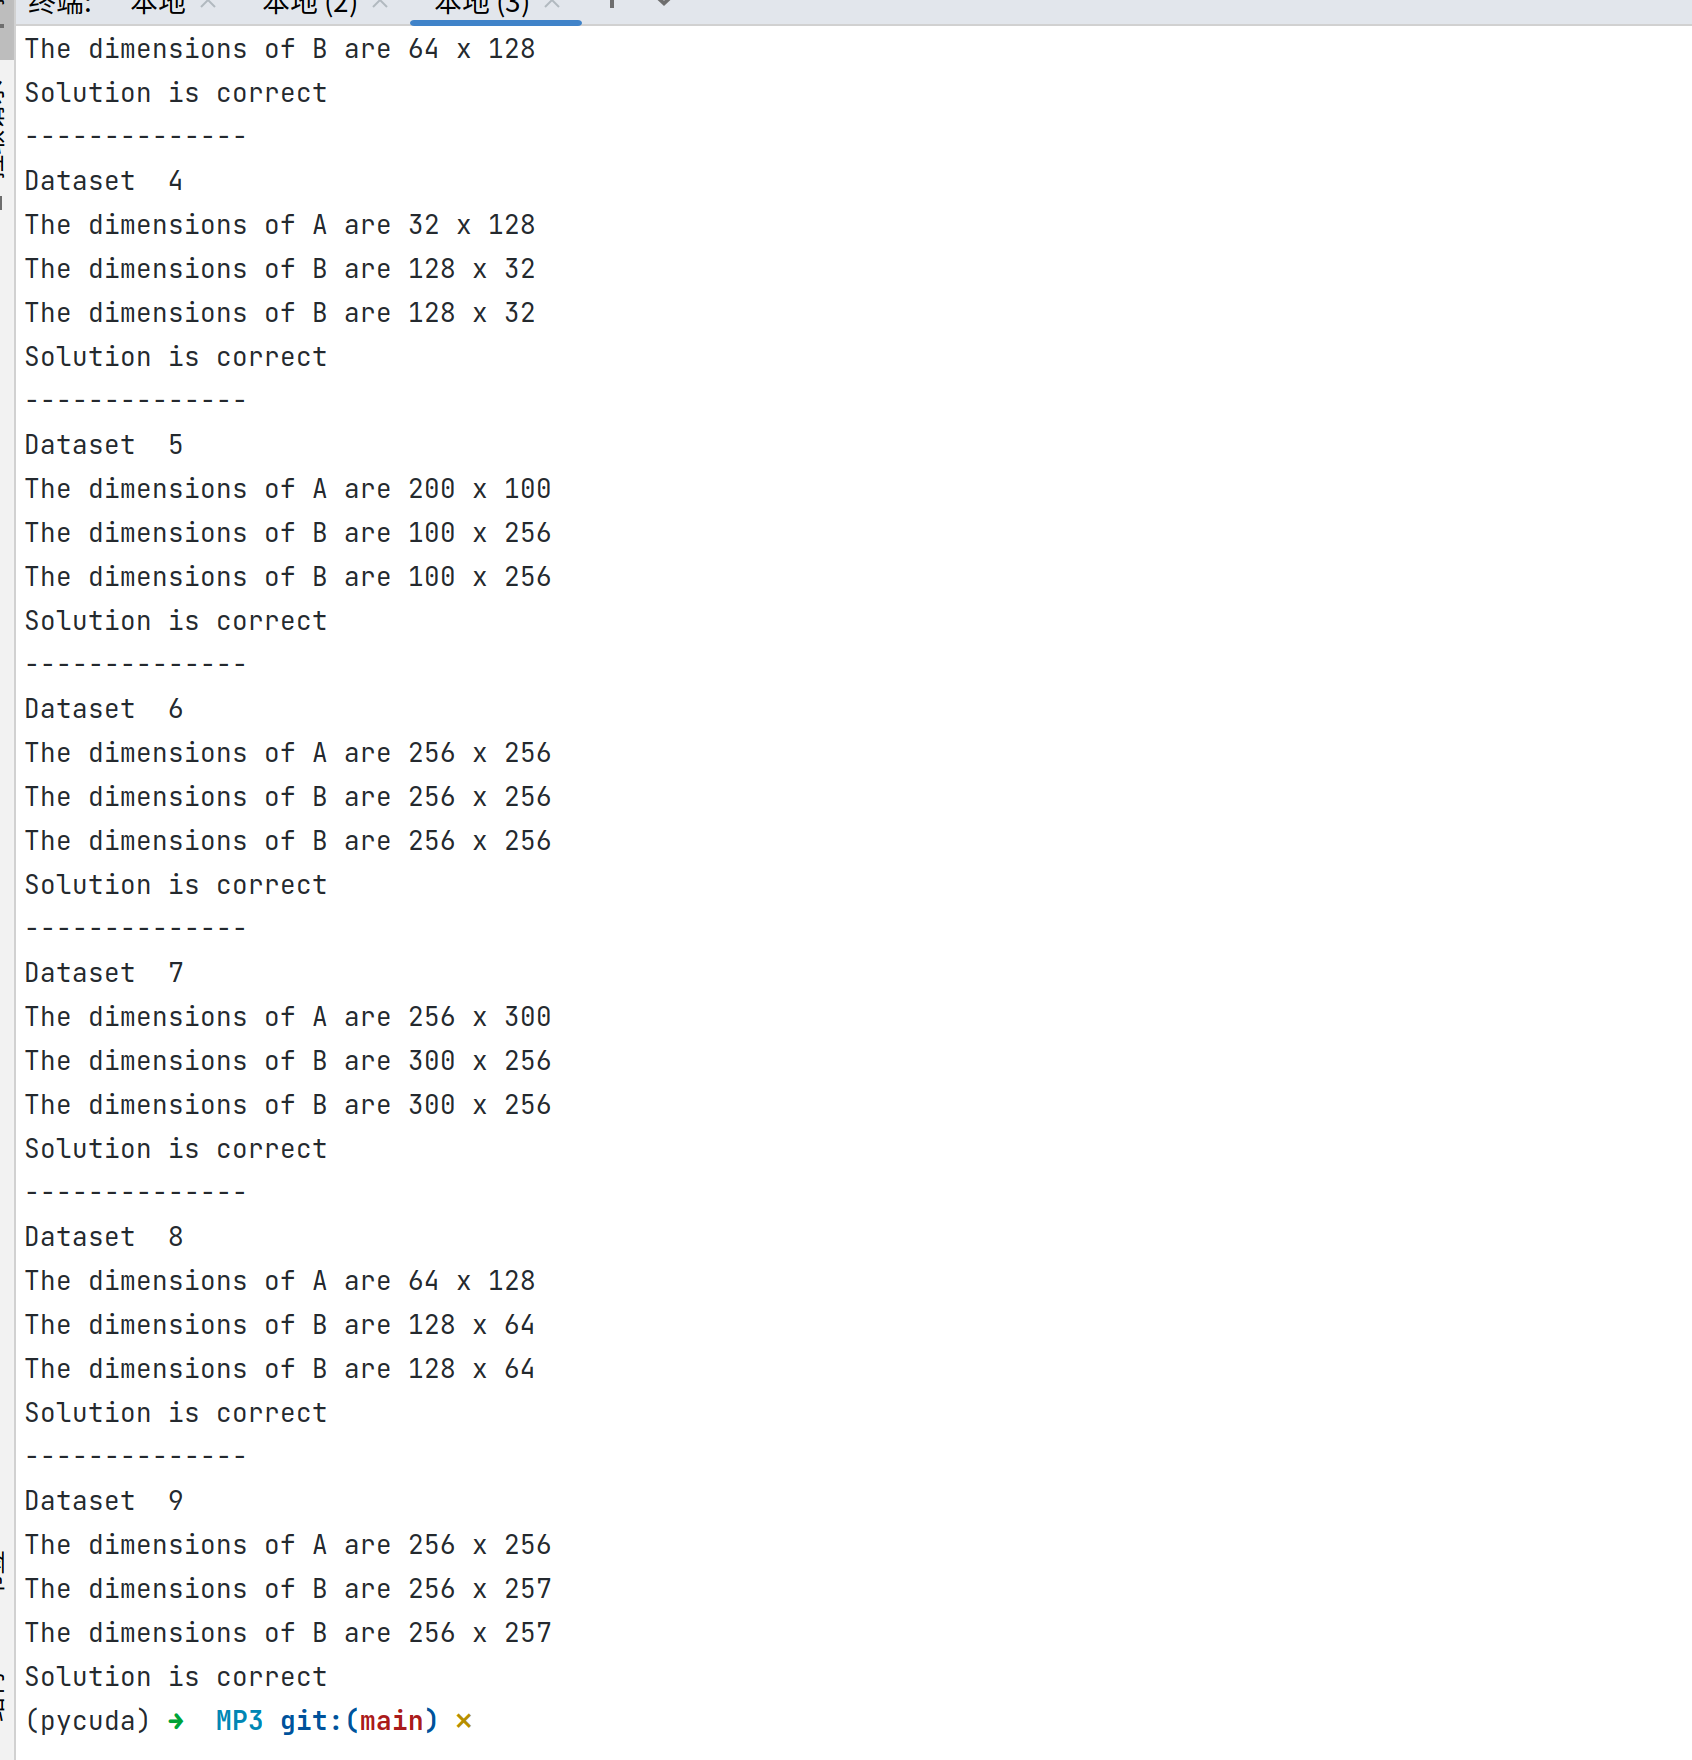
\includegraphics[width=0.8\textwidth]{images/Lab3.png}
	\caption{lab3实验结果}
	\label{fig:1}
\end{figure}

\end{document}